\documentclass[border=2pt]{standalone}
\usepackage{diagrams}
\tikzset{
  edge/.style={line width=1pt},
  vlbl/.style={font=\normalsize},
  elbl/.style={font=\small},
  dotnode/.style={circle, fill=black, inner sep=2pt},
}
\usetikzlibrary{patterns,angles,quotes,arrows.meta,math,calc}
\usepackage{amsmath}
\begin{document}
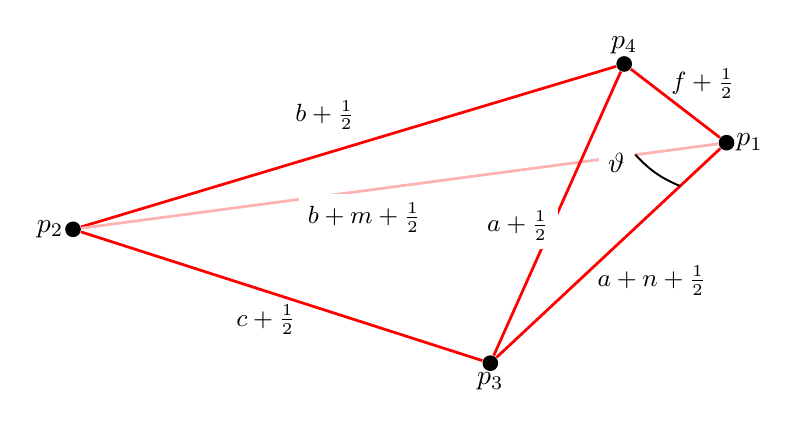
\begin{tikzpicture}[scale=1.0]
  \node[dotnode] (p2) at (-4.6,-0.2) {};
  \node[dotnode] (p4) at ( 2.4, 1.9) {};
  \node[dotnode] (p1) at ( 3.7, 0.9) {};
  \node[dotnode] (p3) at ( 0.7,-1.9) {};

  % six edges
  \draw[edge,color=red] (p2)--(p4);           % b+1/2
  \draw[edge,color=red] (p4)--(p1);           % f+1/2
  \draw[edge,color=red] (p2)--(p3);           % c+1/2
  \draw[edge,color=red!30] (p2)--(p1);           % b+m+1/2
  \draw[edge,color=red] (p3)--(p1);           % a+n+1/2
  \draw[edge,color=red] (p3)--(p4);           % a+1/2

  % angle theta at p1 between edges p1-p3 (a+n+1/2) and p1-p2 (b+m+1/2)
  \path (p1) -- (p3) coordinate[pos=0.18] (t3);
  \path (p1) -- (p2) coordinate[pos=0.13] (t2);
  \draw[line width=0.7pt] (t3) to[bend left=12] (t2);
  \node[vlbl,fill=white] at ($(p1)+(-1.4,-0.25)$) {$\vartheta$};

  % vertices
  \node[vlbl,left]  at (p2) {$p_2$};
  \node[vlbl,above] at (p4) {$p_4$};
  \node[vlbl,right] at (p1) {$p_1$};
  \node[vlbl,below] at (p3) {$p_3$};

  % edge labels
  \node[elbl] at (-1.4, 1.25) {$b+\tfrac12$};
  \node[elbl] at ( 3.4,1.65) {$f+\tfrac12$};
  \node[elbl] at (-2.15,-1.35){$c+\tfrac12$};
  \node[elbl,fill=white] at (-0.9,-0.05) {$b+m+\tfrac12$};
  \node[elbl,fill=white] at ( 1.05,-0.15) {$a+\tfrac12$};
  \node[elbl] at ( 2.75,-0.85) {$a+n+\tfrac12$};
\end{tikzpicture}
\end{document}